%File: formatting-instruction.tex
\documentclass[letterpaper]{article}
\usepackage{epsfig}
\usepackage{graphicx}
\usepackage{url}
\usepackage{aaai}
\usepackage{times}
\usepackage{helvet}
\usepackage{courier}
\usepackage{color}

\newcommand{\red}[1]{\textcolor{red}{#1}}

\frenchspacing
\setlength{\pdfpagewidth}{8.5in}
\setlength{\pdfpageheight}{11in}
\pdfinfo{
/Title (Insert Your Title Here)
/Author (Put All Your Authors Here, Separated by Commas)}
\setcounter{secnumdepth}{0}  
 \begin{document}
% The file aaai.sty is the style file for AAAI Press 
% proceedings, working notes, and technical reports.
%
\title{Identifying Duplicate and Contradictory Information in Wikipedia}
% with Near-Duplicate Sentence Detection}
\author{
BLINDED FOR REVIEW
%AAAI Press\\
%Association for the Advancement of Artificial Intelligence\\
%2275 East Bayshore Road, Suite 160\\
%Palo Alto, California 94303\\
}
\maketitle
\begin{abstract}
\begin{quote}
Our study identifies Wikipedia articles that contain
highly-similar content by applying techniques for near-duplicate
detection at the sentence level. This is accomplished with a MapReduce
implementation of minhash, a locality-sensitive hashing technique, to
identify clusters of sentences with high Jaccard similarity. Analysis
shows that these cluster can be categorize into six different types, two
of which are particularly interesting:\ identical sentences
quantify the extent to which content in Wikipedia is copied and
pasted, and near-duplicate sentences that state contradictory facts
point to quality issues in Wikipedia articles.
\end{quote}
\end{abstract}

\section{Introduction}

Readers of Wikipedia often notice that multiple articles contain
highly-similar or even identical passages. In some cases they represent
duplicate articles that require merging, but content overlap arises
naturally as well. For example, the article about a hurricane and the
article about the location where it made landfall might share the same
content about the impact of the natural disaster. Identical content is
most likely the result of copy and paste between articles, but
interestingly, readers occasionally come across highly-similar content that
state contradictory facts. In a distributed environment where anyone can
edit content, these observations are perhaps not surprising, 
%but we are not aware of any formal studies. 
but in this paper we attempt to
rigorously characterize these phenomena by treating the
problem as that of near-duplicate sentence detection. We
adapt standard locality-sensitive hashing (LSH) techniques to identify
clusters of near-duplicate sentences in Wikipedia.

We believe this problem is interesting in a few ways:\ 
For duplicate sentences,
our analyses quantify the extent to which Wikipedia content is simply
{\it replicated}, as opposed to {\it written} from scratch. 
In the case of {\it near} duplicates, some differences represent
minor copyediting that do not change the substance of the content, but
in other case the differences 
represent contradictory facts. Quantifying these cases
provides an indirect measure of the quality of Wikipedia in terms of
self consistency. We could imagine a robot that continuously monitors
Wikipedia to flag these inconsistencies and requests editors
to intervene and resolve.

This work makes no claims about the novelty of our
techniques nor our implementation for near-duplicate sentence
detection. Rather, our contribution lies in using existing techniques
to analyze Wikipedia. To our knowledge, we have not seen
near-duplicate detection applied to Wikipedia in this way before.

\section{Related Work}

The problem we tackle in this paper is related to a few other problems
that have been studied before. Near-duplicate detection is important
in web search because web pages are often copied or mirrored with only
minor differences (e.g., ads or navigation bars); it would be
desirable to return only the ``canonical'' version in search
results. In fact, the algorithm that we use in this paper,
minhash~\cite{broder:resemblance}, was originally developed for
near-duplicate detection of webpages. Another closely-related problem
is plagiarism detection~\cite{}, or more generally, ``text
reuse''~\cite{seo:dct,bendersky:timeline}. In contrast to near-duplicate detection, the
focus is usually on smaller segments of text as opposed to entire
documents. However, similar approaches such as shingling are
applicable to both problems.

Other similar manifestations of the problem are what the data mining
community calls pairwise similarity search or ``all pairs''
search~\cite{Bayardo_etal_WWW2007} and what the database community
calls set similarity join~\cite{Vernica_etal_SIGMOD2010}. The idea is the same:\ given a
potentially large collection of objects, identify all pairs whose
similarity is above a threshold according to some similarity metric
(e.g., cosine similarity).

There are two large classes of solutions for the above problems:\ in
the {\it index-based} approach, an inverted index is constructed from
objects in the collection and a traversal of this index allows the
similiar pairs to be extraced,
e.g.,~\cite{Bayardo_etal_WWW2007,lin:brute}; with {\it hash-based}
approach, the basic idea is to use locality-sensitive hashing (LSH) to
identify similar pairs based on hash collisions, e.g., minhash~\cite{broder:resemblance}
and others~\cite{}. Of course, hybrid solutions are also
possible. Previously, scaling up of these solutions has been
accomplished by MapReduce~\cite{zhang:pdc,lin:brute,Vernica_etal_SIGMOD2010}. Our approach
take advantage of minhash using a straightforward MapReduce
implementation in Hadoop.

Because of its open nature, Wikipedia has a history of generating
controversy over editorial quality and factual correctness. Although
some studies have found Wikipedia's accuracy to rival that of
traditional encyclopedias, other studies have found numerous factual
errors.[References??] Since Wikipedia may be edited anonymously,
information may freely copied between web sources and even between
Wikipedia articles without verification. Additionally, many articles
in Wikipedia lack citations. Although there are active communities of
editors who contribute to the upkeep of various articles, often
focusing on a partiular subject area and expanding and improving the
related content, still much of Wikipedia content is created in an
unsupervised manner. Wilkinson found the distribution of article edits
on Wikipedia to have a long tail, meaning that a small number of
articles have many edits while most articles have few, and that the
number of edits is directly related to article quality. Articles with
low edits and low editorial attention, are less likely to be updated
when new information is available \cite{wilkinson:wiki}.

\section{Near-Duplicate Detection}

In order to measure document similarity we use a common LSH technique
known as MinHash \cite{broder:resemblance}. A minhash signature on a
text document is calculated using a parametrized family of hash
functions $F_i$, $1 \le i \le N$. (In our case, input ''documents''
are individual sentences found within the content of Wikipedia
articles.) Each document is broken up into n-gram ``shingles'' and for
each shingle set $S$ a set $\{min_{s \in S}(F_i(s)\}$ of minimum
hashes over the hash family is produced. The signature on a document
$d$ is represented as a vector of $K$ minhashes, chosen from the set
$\{min_{s \in S}(F_i(s)\}$ of minimum hashes. In order to minimize
false negatives we generate multiple signatures ($M$ signatures) for
each input sentence.

$K$, $N$, $M$, $n$, as well as the size in bits of the
hashes are all parameters that must be set for the minhash algorithm.

\red{I think I misunderstood banding (which appears to be hashing of
  hash signatures) and it is not what we are doing here, so I took out
  the reference.}

%% \subsection{Design}
%% Many signature techniques such as LSH are embarrassingly parallel. In our project, we designed our algorithm around the MapReduce framework.

%% Because the minhash technique is parametrized by several variables, including shingle length, signature size, and number of signatures to be calculated per document, these values can also be considered as inputs for the MapReduce algorithm.

%% \begin{table}
%% \begin{algorithm}[H]
%% \caption{Minhash MapReduce Pseudocode}
%% \begin{algorithmic}
%% \Function{initialize}{}
%% %\Comment{configure and set up algorithm parameters}
%%  \State $F \gets $ hash family;
%%  \State $L \gets $ shingle length;
%%  \State $K \gets $ vector length;
%%  \State $N \gets $ number of signatures to emit;
%% \EndFunction

%% \Function{map}{docid $d$, wikipage $p$}
%%  \State sentencect $\gets 0$
%%  %\Comment {Break up article text into sentence}
%%  \While{$s \gets$ nextSentence($p$)}
%%   %\Comment{Break up sentence into shingles}
%%   \State shingles $\gets$ shingleSet($s$,$L$);
%%   \State minhashes = new List(|F|);
%%    \For{$i \gets 1 \ldots |F|$}
%%     \State minhashes[$i$] $\gets \infty$;
%%    \EndFor
%%    %\Comment{Calculate set of minhash signature for each sentence}
%%    \For{$g \in$ shingles}
%%     \For{$i \gets 1 \ldots |F|$}
%%      \State minhashes[$i$] $\gets$ min($F_i(g)$,minhashes[$i$]);
%%     \EndFor
%%    \EndFor
%%    %\Comment{Emit $N$ $K$-length signatures}
%%   \For{$i \gets 1 \ldots N$}
%%    \State sig = select($K$, minhahses);
%%    \State emit(sig,(docid,sentencect));
%%   \EndFor
%%   \State  sentencect++;
%%  \EndWhile
%% \EndFunction

%% \Function{reduce}{signature sig, sentenceids $S$}
%% \If{$|S| > 1$}
%% \State emit(sig, $S$);
%% \EndIf
%% \EndFunction
%% \end{algorithmic}
%% \end{algorithm}
%% \end{table}

\subsection{MapReduce Implementation}

In our MapReduce algorithm, the mapper receives a Wikipedia article
(value) that is identified by a unique docid (key). Inside the mapper
we break the article into sentences using a regular expression;
sentences that are shorter than 75 shingles words or longer than 600
shingles are discarded. For each sentence, the minhash signatures are
then computed. The family of hash functions is implemented using a
``Multiply Shift'' hashing scheme\footnote{\small
  http://en.wikipedia.org/wiki/Universal\_hashing} and is generated
from a random seed. The hash family is also parametrized by hash
output key size, which is also configurable. For our experiments we
use a 60 bit hash and a hash family of size 20.

Each signature is emitted as the key of an intermediate key--value
pair with the sentence id as the value (constructed from the docid and
the sentence count).

The MapReduce programming model guarantees that all values associated
with the same key are shuffled to the same reducer---in effect,
collecting the hash collisions for us. In the reducer we receive a
signature as a key and as values all sentence ids that share the
signature. If there is more than one value per key, we write out all
sentence ids as a cluster. This serves as input to the final cluster
generation stage (see below).

\subsection{Parameter Tuning}

The minhash algorithm is parametrized by several values, including
shingle length, length of hash vectors, number of hash signatures per
input document, and hash output size. Each of these parameters has an
impact on the error rates in the minhash output. For our experiments
we choose 10 signatures ($M$ = 10) per input sentence, since sentences
themselves are small and we will be processing many of them. Once we
have fixed $M$ we can use the property that the probability of a match
between two sentences is equal to the Jaccard similarity of their
shingle sets. Thus the probability of a match for two sentences $A$
and $B$ can be expressed as follows:
\[P[match(A,B)] = 1 - (1 - s^K)^M\]
where $s$ = Jaccard($A$,$B$). Here we choose $K = 10$. Given these
settings, if we choose .9 Jaccard similarity as our goal (90\% overlap
in shingle sets), then there is a 99\% chance of a match, while
sentences similarity .7 have only a 25\% chance of being a match and
sentences with similarity .6 have only a 6\% chance of being a match.

With the above settings we can make a conservative estimate of the
amount of data generated by our signature generation code: (60 bit
signatures) $\times$ (10 hashes per signature) $\times$ (10 signatures
per document) $\times$ (10m Wikipedia articles) $\times$ (100
sentences per article) $\approx$ 70GB of minhash output.

We choose a shingle length of 12 with the goal of shingle sets that
cross word boundaries in order to preserve sentence order.

Observe that it is possible to improve precision by filtering results
with secondary testing on the output signature groups, thus allowing
one to improve recall by relaxing parameters. The current work does
not investigate parameter tuning with filtering.

\red{Is this sufficient discussion for recall? The probability curve gives us a recall estimation at each level of similarity, which I think is better than an overall recall estimation via experiment.}

\begin{figure}
\centering
\includegraphics[width=3.25in, keepaspectratio = true]{jacmatchprobs.png}
\caption{Minhash Parameter tuning.}
\label{clust}
\end{figure}

\subsection{Final Cluster Generation}

The output of our minhash algorithm is a set of clusters, where each
cluster represents a signature collision. Since we generate multiple
signatures per document, it is possible (and frequently observed) that
a sentence appears in multiple clusters. We adopt the standard
practice of merging all clusters that share at least one common
sentence. (If we were applying secondary filtering to remove false
positives, it would make sense to apply it before merging clusters.)
Cluster merging is accomplished in one pass with a union find data
structure. In union find each node maintains a pointer to a head node
for the set. We maintain a lookup table from each sentence id to its
node in the union find structure. As we read the input clusters we
look up the node for each sentence as merge clusters or create new
ones as needed. Merging two clusters involves changing the head node
of one cluster to point to the head of the other. In practice when
walking up the tree to find the head we change all nodes along the way
to point to the head node to reduce search time. Once clusters are
merged we do a pass over our lookup table to obtain the mapping from
clusters to nodes.

\subsection{Mapping Back to Sentences}

Once we have merged clusters we typically wish to map the sentence ids
back to their corresponding text so that we can analyze the content of
each cluster. To accomplish this we use another MapReduce job that
reads the merged cluster output as side data and creates a hashmap
from the original docid (contained in the sentenceid) to a
sentence/cluster pair. The MapReduce job maps back over the original
Wikipedia data, using the same regular expression to break up
documents into sentences. For each input sentence, the mapper checks
to see if the sentence is in the cluster hashmap. If so, it emits a
key value pair with the cluster id as the key and an (article title,
sentence text) pair as the value. Once again, the MapReduce framework
takes care of grouping output by key so that sentences in the same
cluster are grouped together. Since no further processing is necessary
for the clusters, we use the identify reducer, which passes on the
keys and values as received.

\begin{figure}
\centering
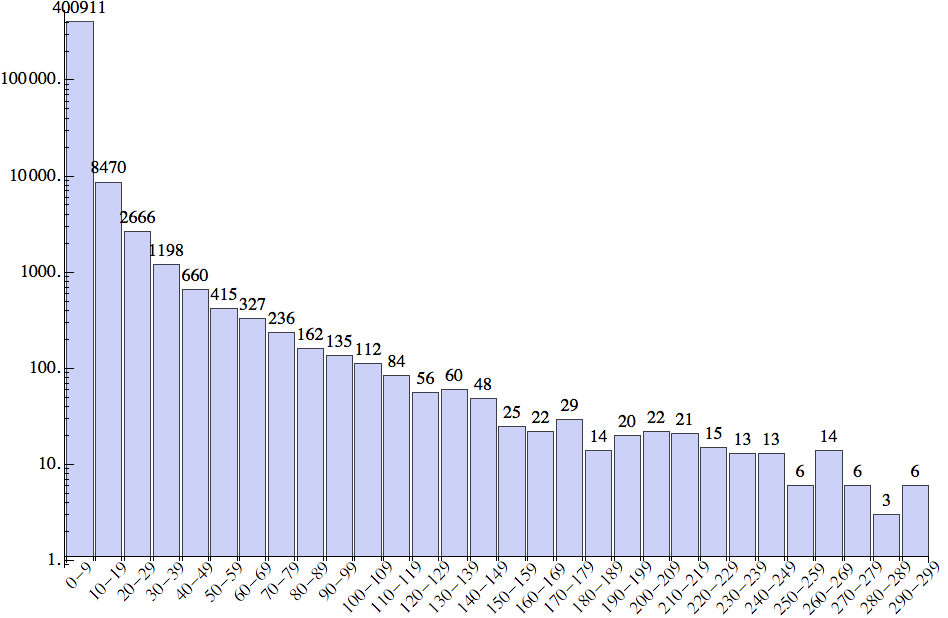
\includegraphics[width=3.25in, keepaspectratio = true]{clusterhistogram.png}
\caption{Histogram of Cluster Sizes.}
\label{params}
\end{figure}

\section{Experimental Results}

Our analysis was conducted on an XML dump of English Wikipedia from
July 2013. The entire corpus is approximately 42 GB and contains 10.2m
articles (after excluding certain non-article pages). Based on our
simple sentence chunker, there are a total 135.8m sentences in the
corpus.

Running our Hadoop implementation of minhash on the entire collection
took approximately 25 minutes on our cluster consisting 16 nodes (128
cores). Code necessary for replicating these experiments have been
made open source.\footnote{\small BLINDED}

%https://github.com/seweissman/wikiduper}.

After the processing pipeline, we identified 1.15m clusters, 3.50m
article/sentence pairs over 1.09m articles. The clusters contain 2.36m
unique sentences in total. Cluster sizes range from 2 to 42,901; see
Figure~\ref{clust} for histogram. Most clusters are small; about 99\%
of the clusters have sizes less than or equal to ten, but about a
quarter of the output sentence/article pairs fall into clusters with
size greater than ten. 

Of the 14,488 clusters greater than size 10, 2722 (18.8\%) contain
identical sentences. 3890 (26.8\%) have fewer than 50\% of their
sentences unique. 5725 contain entirely unique sentences. Manual
inspection shows that many of the large clusters, including most of
the clusters of entirely unique sentences consist of ``template''
sentences, where sentences follow strict patterns of construction (See
discussion of sentence types below). Non-unique clusters consist of
such templates, but also largely identical groupings of sentences
where some of the sentences have been edited, e.g. the following
cluster contains 663 sentences, 661 of which are identical

\red{I can confirm the relation between large clusters and templates by looking at results, but cannot confirm that template articles are mostly stubs. I guess it would be possible to look at whether articles in large clusters have shorter length on average.}

\begin{itemize}
\item They are capable of "stinging" humans therefore live ones should be handled carefully or not at all. [661 sentences]
\item They are capable of "stinging" therefore live ones should be handled carefully or not at all. [1 senence]
\item They are capable of "stinging" humans; therefore live ones should be handled carefully or not at all. [1 sentence]
\end{itemize}

Other clusters show distributions of sentences that imply that appear to reflect more complex editing patterns. E.g., the following sentences are part of a cluster of size 299. Each is plausibly a variation of one original sentence that has been edited and replicated multiple times:

\begin{itemize}
\item In the Commonwealth of Pennsylvania pension and Social Security income are exempted from state personal income tax and local earned income tax regardless of the individual's wealth. [67 sentences]
\item In the Commonwealth of Pennsylvania pension income and Social Security income are exempted from state personal income tax and local earned income tax regardless of the level of the individual’s personal wealth. [63 sentences]
\item In the Commonwealth of Pennsylvania pension income and Social Security income are exempted from state personal income tax and local earned income tax regardless of the individual's level of wealth. [18 sentences]
\item In Pennsylvania pension income and Social Security income are exempted from state personal income tax and local earned income tax regardless of the level of wealth. [15 sentences]
\item In the Commonwealth of Pennsylvania pension income and Social Security income are exempted from state personal income tax and local earned income tax regardless the of income level. [13 sentences]
\item In the Commonwealth of Pennsylvania pension income and Social Security income are exempted from state personal income tax and local earned income tax regardless of the person's wealth. [12 sentences]
\end{itemize}


%\subsection{Similar Sentence Types}

\begin{figure*}[t]
{\small
{\bf Templates}\\
Of the agricultural land 40.4\% is used for growing crops and 26.6\% is pastures while 2.2\% is used for orchards or vine crops. [Gondiswil] \\
Of the agricultural land 26.1\% is used for growing crops and 30.2\% is pastures while 3.0\% is used for orchards or vine crops. [Kleindietwil] \\
Of the agricultural land 37.8\% is used for growing crops and 35.5\% is pastures while 2.2\% is used for orchards or vine crops. [Leimiswil] \\[1ex]
{\bf Identical}\\
Professional organizers help redirect paradigms into more useful cross-applications that ensure properly co-sustainable futures for their clients' spaces and processes. [Professional organizing] \\
Professional organizers help redirect paradigms into more useful cross-applications that ensure properly co-sustainable futures for their clients' spaces and processes. [Professional organizer] \\[1ex]
{\bf Copyediting}\\
In dry areas it may only emerge from its burrow for a few weeks when conditions are right and usually at night but in areas with permanent water bodies and abundant rain it may be active all day. [Great Plains toad] \\
In dry areas it may only emerge from its burrow for a few weeks when conditions are right and only at night but in areas with permanent water bodies and abundant rain it may be active all day. [List of amphibians and reptiles of Montana]\\[1ex]
{\bf Factual Drift}\\
The color of the upper rim of an astronomical object could go from green to blue to violet depending on the decrease in concentration of pollutants as they spread throughout an increasing volume of atmosphere. [Green flash] \\
The color of the upper limb of an astronomical object could go from blue to green to violet depending on the decrease in concentration of pollutants as they spread throughout an increasing volume of atmosphere. [Mirage of astronomical objects] \\[1ex]
{\bf References}\\
Neotropical Ichthyology 11 (1): 73-80. \\
Neotropical Ichthyology 10 (2): 245-253. \\[1ex]
{\bf Other}\\
Army Medical Research Institute of Infectious Diseases (USAMRIID) microbiologist Bruce E. [Timeline of the 2001 anthrax attacks] \\
Army Medical Research Institute of Infectious Diseases (USAMRIID) which transitioned from the previous U.S. [Fort Detrick]}
\caption{Categories of near-duplicate sentences in Wikipedia.}
\label{toparticlegroups}
\end{figure*}

Based on manual inspection of cluster output, we can categorize
near-duplicate clusters into one of six types. Examples are shown in
Figure~\ref{toparticlegroups} %(with article titles in brackets) 
and discussed below.

\emph{Templates} describe sentences that have identical structure, but
with different entities, facts, or figures for {\it different} topics
(and thus are not contradictory). They reflect conscious attempts to
impose structure across groups of articles that may be related. Since
several of the largest template clusters contain tens of thousands of
sentences (the largest over 40,000), it is likely that some
template groups are automatically generated using bots.

\emph{Identical} sentences are the result of copy and paste, and are
often found in articles that cover similar topics or articles that are
subtopics of other topics.

Non-identical but highly-similar sentences break down into two types:
\emph{Copyediting} refers to nearly identical sentences that differ in
stylistic or otherwise non-substantive ways. They arise with minor
editing after a copy and paste. \emph{Factual drift} describes
sentences about the {\it same} topic that provide contradictory
facts. Although without detailed research, there is no way to
ascertain which version (if any) is correct, we can identify a common
scenario. After a copy and past, a fact becomes out of date (e.g., the
tallest building or the death toll in a disaster) and is corrected in
one instance but not the others.

\emph{References} refers to citations, typically occurring at the end
of articles. Since Wikipedia does not adhere to one single citation
style, the same work may be cited differently, or multiple citations
to the same venue may be similar.

Finally, all clusters that do not fit into any of the above category
are classified as \emph{other}. These typically represent sentences
that are highly similar, but otherwise bear no semantic relationship
with each other. Sentence chunking errors often contribute to these
spurious results.

%\subsection{Breakdown of Sentence Types and Filtering}

To quantify the distribution of these six cases, we randomly sampled
2094 clusters and performed manual classification. The results are
shown in Table~\ref{counts}. Nearly three quarters of all clusters
are either \emph{identical} or the \emph{template}.


\begin{table}
\centering
\caption{Sentence Breakdown Counts}
\vspace{0.2cm}
\begin{tabular}{| l | r | r |}
\hline
type & count & fraction \\
\hline
\hline
Templates     & 632 & 30.18\% \\ \hline
Identical     & 948 & 45.27\% \\ \hline
Copyediting   & 283 & 13.51\% \\ \hline
Factual drift & 121 &  5.78\% \\ \hline
References    &   7 &  0.33\% \\ \hline      
Other         & 103 &  2.92\% \\ \hline
\end{tabular}
\label{counts}
\end{table}

\section{Future Work and Conclusions}

Currently, our technique only identifies clusters of sentences that
are above a certain threshold in Jaccard similarity. Missing from our
analysis is the notion of information flow:\ Which was the source
article and which was the target? Are there copy ``chains'' where
content was progressively copied from one article to the next, with
possible ``branches''? This information 

\red{Need to rework rest...}

Although the LSH technique of minhashing does not perfectly approximate edit distance, we have demonstrated that, when implemented in the Hadoop framework, it is an efficient method for identifying large numbers of Wikipedia sentences that are near duplicates. Additionally, we demonstrated that it is possible to apply a simple heuristic and to filter sentences that result from templatification, which make up about half (by our heuristic scoring) of the sentences identified in the similar sentence analysis. Because templatification appears quite often as almanac-like lists of facts, quite possibly generated with automated ``bots'' given the large scale of some templatified clusters, it is a worthwhile exercise to identify and quantify such content as distinct from other content found on the Wikipedia site.

Although sentences can be used as a measure of article similarity, identifying similarity at the sentence level allows greater flexibility for finding similar content across documents than a whole document analysis. These techniques could be used to automatically suggest corrections to Wikipedia, or to improve plagiarism detection across web content in general.

Future work could investigate revision histories of articles and correlate similar sentence with article edit timestamps to better relate similarities on a temporal dimension. An analysis on a multi-sentence level could identify more similarities where user edits change sentence boundaries by merging or breaking up content which our present analysis would not detect. Additionally, a more sophisticated template detection heuristic could be developed, as the one used here is a very rough measure that makes assumptions specific to English language text.

%\section{Acknowledgments}
%We would especially like to thank Dr. Jimmy Lin for his advise and directions.

\bibliographystyle{aaai}
\small
\bibliography{wikisentences} 

\end{document}
